


 

 
%\section{Struktogramm}

%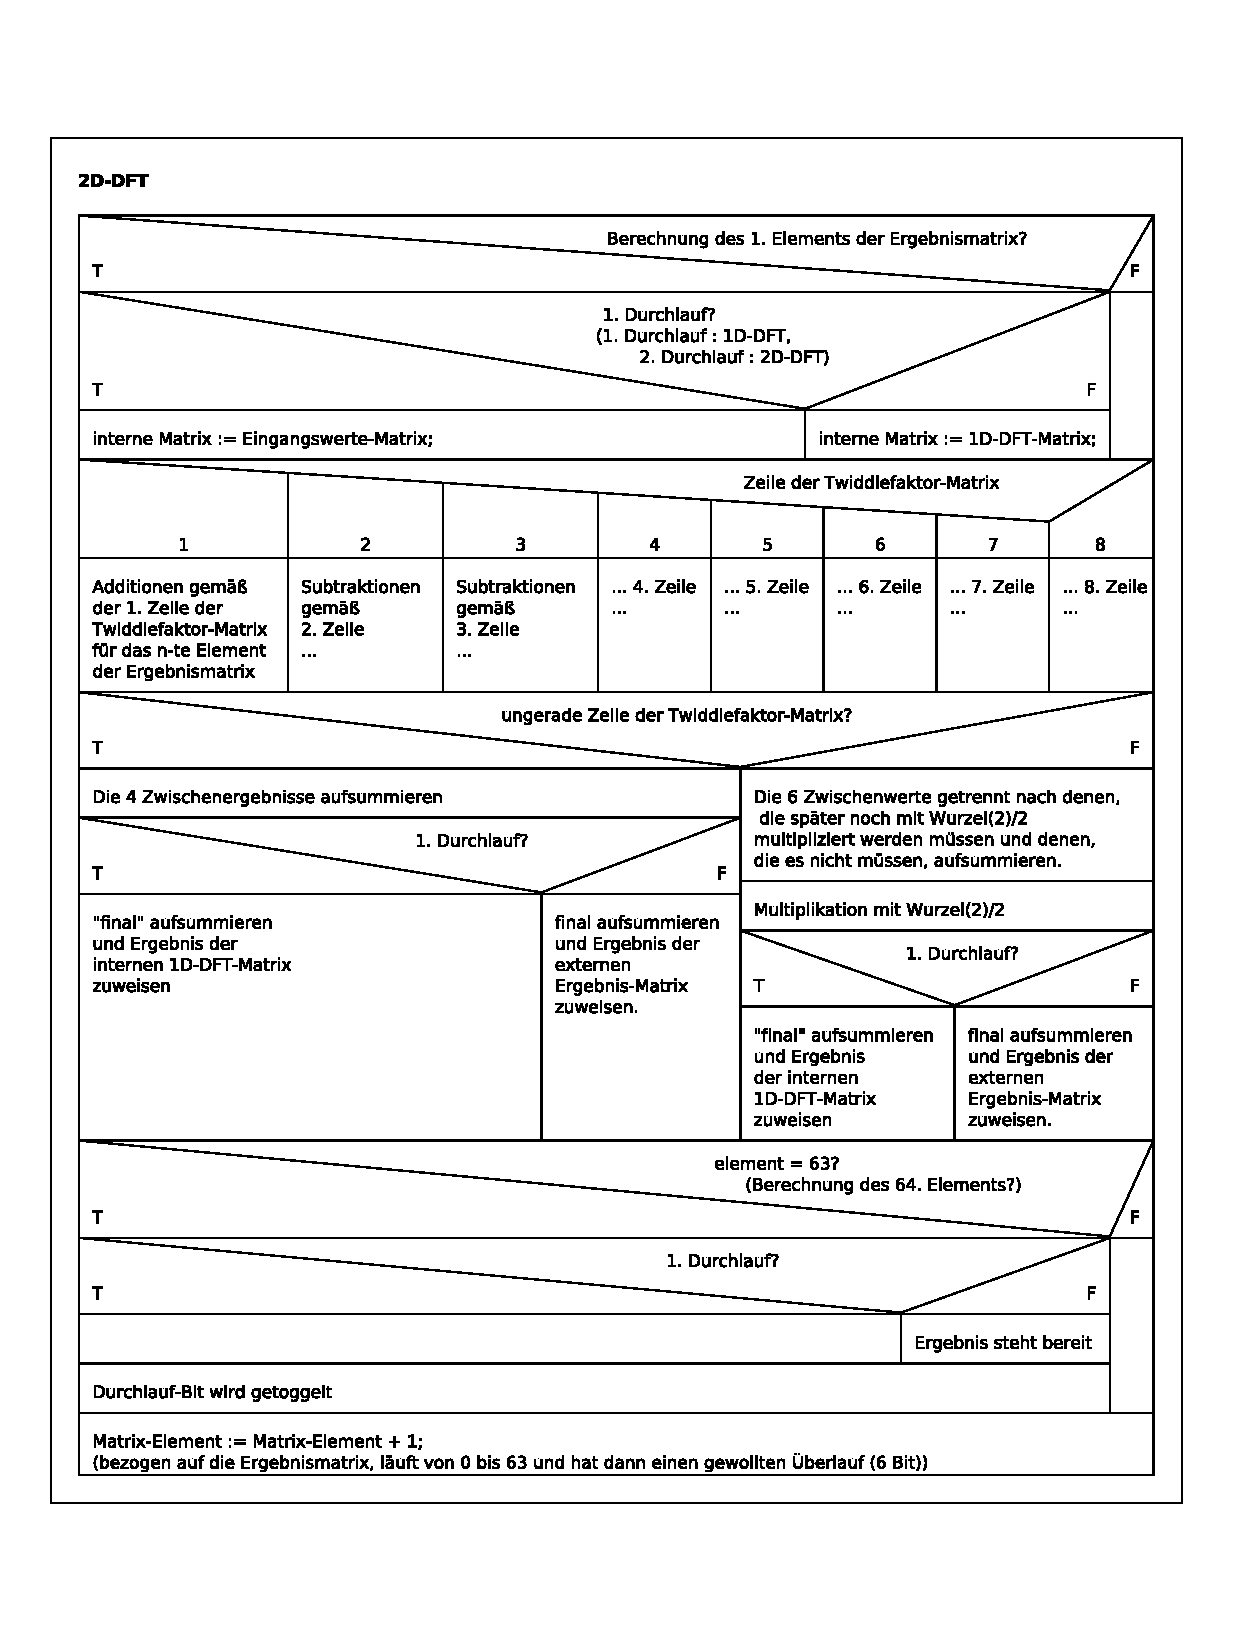
\includepdf{content/Struktogramm.pdf}

\section{Schema der Zustandsfolge}
In Abbildung \ref{pic:Automatengraf} sind die Zustände des in VHDL implemetierten Zustandsautomaten zu sehen. Da es sich um einen sehr strikten Ablauf handelt und
keine Eingangssignale Einfluss auf die Zustandsfolge haben, wurde sich gegen die Darstellung als klassichen Automatengraph entschieden. 
Stattdessen ist in Abschnitt \ref{sec:UML-Diagramm} ergänzend das UML-Diagramm mit der detaillierten Abfolge der Berechnung zu sehen, welches einen wesentlich höheren 
Informationsgehalt besitzt. Es wurde so gestaltet, dass daraus hervorgeht, welches der aktuelle Zustand ist.


\begin{figure}[t!]
 \centering
\begin{tikzpicture}[->,>=stealth',shorten >=1pt,auto,node distance=4.9cm,
                    semithick,initial text=nReset, initial where=above, text width=3cm, align=center]
  \tikzstyle{every state}=[fill=white, text=black]
  %\tikzstyle{every initial where}=[above]
  

  \node[initial,state, circle split,minimum size=10pt] (A)                   {Idle \nodepart{lower} {}\\ \_\_\_};
  \node[state, circle split, minimum size=65pt]         (B) [below right of=A]{Twiddle\_Calc \nodepart{lower} {}\\ \_\_\_};
  \node[state, circle split, minimum size=65pt]         (C) [below right of=B]      {Additions\_1 \nodepart{lower} {}\\ \_\_\_};
  \node[state, circle split, minimum size=65pt]         (D) [below of=C] {Additions\_2 \nodepart{lower} {}\\ \_\_\_\_};
  \node[state, circle split, minimum size=65pt]         (E) [below left of=D] {Const\_mult \nodepart{lower} {}\\ \_\_\_};
  \node[state, circle split, minimum size=65pt]         (F) [above left of=E]      {Additions\_3 \nodepart{lower} {}\\ \_\_\_};
  \node[state, circle split, minimum size=65pt]         (G) [above of=F]      {set\_ready\_bit \nodepart{lower} result\_ready=1};

  
   \path (A) edge (B) 
         (A) [loop left] edge(A)
         (B) [bend left=10] edge (C)
         (C) edge (D)
         (D) edge node [sloped, anchor=center, below]{element(3)=0}(B)
         %(D) edge node [sloped, anchor=center, below]{element(3)=1}(E)
         (D) edge node [right=1.1cm, anchor=center, below]{element(3)=1}(E)
         (E) edge (F)
         (F) [bend right=10] edge node [sloped, anchor=center, below]{element<63 $\vee$ dft\_1d\_2d=0 }(B)
         (F) [bend left=10] edge node[left]{element=63 $\wedge$ dft\_1d\_2d=1}(G)
         %(G) edge node [above left] {result\_ready=1} (B);
         (G) edge (B);
\end{tikzpicture}
\caption{Zustandsfolge der Berechnung der 1D- bzw. 2D-DFT.}
\label{pic:Automatengraf}
\end{figure}

Der Zustand \texttt{set\_ready\_bit} wird nach dem zweiten Durchlauf der DFT-Einheit, also wenn die 2D-DFT berechnet ist, erreicht. Dieser setzt für einen Takt
das Signal \texttt{result\_ready} auf Eins.
Wenn \texttt{element(3)=0} ist, ist es eine ungerade Zeile der Twiddlefaktormatrix. \texttt{dft\_1d\_2d=0} besagt, dass die 1D-DFT berechnet wird.
\section{UML-Diagramm}\label{sec:UML-Diagramm}

% Define block styles
\tikzstyle{decision} = [diamond,                    draw, fill=blue!20, text width=6em, text badly centered, node distance=4cm, inner sep=0pt]
\tikzstyle{block} =    [rectangle, rounded corners, draw, fill=blue!20, text width=5em, text centered,       node distance=4cm, minimum height=5em, minimum width=7em]
\tikzstyle{smallblock} =    [rectangle, rounded corners, draw, fill=blue!20, text width=5em, text centered,       node distance=4cm, minimum height=2em, minimum width=3.5em]
\tikzstyle{wideblock} =    [rectangle, rounded corners, draw, fill=blue!20, text width=7em, text centered,       node distance=4cm, minimum height=5em, minimum width=7em]
\tikzstyle{verywideblock} =    [rectangle, rounded corners, draw, fill=blue!20, text width=15em, text centered,       node distance=4cm, minimum height=4em, minimum width=15em]
\tikzstyle{textblock} =    [rectangle, rounded corners, draw, fill=blue!20, text width=12em, text centered,       node distance=4cm, minimum height=4em, minimum width=10em]
\tikzstyle{dot}=[draw,shape=circle]

\tikzstyle{arrowline} = [draw, -latex']


    
\begin{tikzpicture}[auto, node distance = 1cm and 1cm, initial text=POR, initial where=above]
    % Place nodes
    \node [initial, smallblock] (start) {Idle};
    \node [decision, below of=start, node distance=3cm] (init) {IDFT?};
    \node [block, below right of=init, node distance=3cm] (Zeilenindex) {Zeilenindex tauschen};
    \coordinate[below of=init, node distance=3.5cm](Punkt_0);
    \node [decision, below of=Punkt_0, node distance=2cm] (Element_1) {Berechnung 1. Element?};
    \coordinate [right of=Element_1, node distance=4cm](c1);
    \node [decision, below of=c1, node distance=2cm] (Berechnung_1D_1) {Berechnung 1D-DFT?};
    
    \node [block, below of=Berechnung_1D_1, node distance=3cm] (überschreiben_mit_eingangswerten) {Zwischen- werte := 1D-DFT-Werten};
    \node [block, right of=überschreiben_mit_eingangswerten, node distance=4cm] (überschreiben_mit_1D_Werten) {Zwischen- werte := Eingangswerte};
    \node [block, left of=überschreiben_mit_eingangswerten, node distance=4cm] (Werte_beibehalten) {Zwischen- werte := Zwischen- werte};
    
    \node [dot, fill, inner sep=1pt, below of=überschreiben_mit_eingangswerten,node distance=1.5cm] (Punkt_1){};
    \node [decision,                 below of=Punkt_1,node distance=2cm] (Zustandsabfrage) {Zeilen- abfrage};
    
    \node [dot, fill, inner sep=1pt, below of=Zustandsabfrage,node distance=2cm] (Punkt_2){};
    \coordinate[below of=Punkt_2, node distance=0.5cm](Punkt_3);
    
    \node [textblock, right of=Punkt_2, node distance=3cm] (Zeile_1){Berechnungen entsprechend Zeile 1 der Twiddlefaktor-Matrix};
      
    \coordinate[below of=Punkt_3](Punkt_4);
    \coordinate[below of=Punkt_4,node distance=0.5cm] (Punkt_5);
    \node [textblock, right of=Punkt_5, node distance=3cm] (Zeile_8){Berechnungen entsprechend Zeile 8 der Twiddlefaktor-Matrix};
    
    \coordinate[right of=Zeile_1, node distance=3cm](Punkt_6);
    \coordinate[below of=Punkt_6, node distance=0.5cm] (Punkt_7);
    \node [dot, fill, inner sep=0.01pt, right of=Zeile_8, node distance=3cm](Punkt_9){};
    \coordinate[above of=Punkt_9, node distance=0.5cm] (Punkt_8);
    \coordinate[below of=Punkt_9, node distance=2cm](Punkt_10);
    \coordinate[left of=Punkt_10, node distance=12cm](Punkt_return_1);
    
    \coordinate[right of=init, node distance=8cm](textfeld);
    \node [draw, text, fill=white, above of=textfeld, node distance=1.3cm](tf){Zustand 2: Twiddle\_Calc};
    \coordinate[right of=start, node distance=7.1cm](textfeld2);
    \node [draw, text, fill=white, above of=textfeld2, node distance=1cm](tf2){Zustand 1: Idle};
    \node [dot, fill, inner sep=1pt, above of=init, node distance=1.7cm](Knoten_init){};
    
   % Koordinaten für Hintergrund
   \coordinate [above of=start, node distance=1.5cm](b11);
   \coordinate [right of=start, node distance=13.6cm](b12);
   \coordinate [below of=start, node distance=1cm](b13);
   \coordinate [left of=start, node distance=1.5cm](b14);
    
    % Draw edges
    \draw (start) -- (Knoten_init);
    \path [arrowline] (Knoten_init) -- (init);
    \path [arrowline] (init) -| node [near start] {ja} (Zeilenindex);
    \draw (Zeilenindex) |- (Punkt_0);    
    \draw (init) -- node [left, near start] {nein} (Punkt_0);
    \path [arrowline] (Punkt_0) -- (Element_1);
    \path [arrowline] (Element_1) -| node [near start] {ja} (Berechnung_1D_1);
    \path [arrowline] (Berechnung_1D_1) -- node [near start] {nein} (überschreiben_mit_eingangswerten);
    \path [arrowline] (Berechnung_1D_1) -| node [near start] {ja} (überschreiben_mit_1D_Werten);
    \path [arrowline] (Element_1) -- node [left, near start] {nein} (Werte_beibehalten);
    
    \draw (Werte_beibehalten) |- (Punkt_1);
    \draw (überschreiben_mit_eingangswerten) -- (Punkt_1);
    \draw (überschreiben_mit_1D_Werten) |- (Punkt_1);
    \path [arrowline] (Punkt_1) -- (Zustandsabfrage);
    \draw (Zustandsabfrage) -- (Punkt_2);
    
    \path [arrowline] (Punkt_2) -- (Zeile_1);
    \draw (Punkt_2) -- (Punkt_3);
    \draw [loosely dotted] (Punkt_3) -- (Punkt_4);
    \draw (Punkt_4) -- (Punkt_5);
    \path [arrowline](Punkt_5) -- (Zeile_8);
    
    \draw (Zeile_1) -- (Punkt_6);
    \draw (Punkt_6) -- (Punkt_7);
    \draw [loosely dotted] (Punkt_7) -- (Punkt_8);
    \draw (Punkt_8) -- (Punkt_9);
    \draw (Zeile_8) -- (Punkt_9);
    \draw (Punkt_9) -- (Punkt_10);
    %\draw (Punkt_return_1) |- (Knoten_init);
    \path [arrowline] (Punkt_9) -- (Punkt_10);
    \path (start) [loop right] edge (start);
    
     \begin{pgfonlayer}{background}
      \filldraw [fill=gray!20, draw=gray!15]
        (b11.north -| b12.west)  rectangle (b13.south -| b14.east);
     \end{pgfonlayer}

    
\end{tikzpicture}

\begin{tikzpicture}[auto, node distance = 1cm and 1cm, initial text="", initial where=above]



\node [initial, decision] (gerade_Zeile_1) {gerade Zeile?};
\node [wideblock, below left of=gerade_Zeile_1] (gerade_Zeile_1_aufsummieren) {Zwischenwerte paarweise aufsummieren};
\node [wideblock, below right of=gerade_Zeile_1] (ungerade_Zeile_1_aufsummieren) {Zwischenwerte paarweise aufsummieren, zu multiplizierende getrennt};
\node [dot, fill, inner sep=1pt, below of=gerade_Zeile_1, node distance=5cm](Punkt_1){};


\node [decision, below of=Punkt_1, node distance=4cm] (gerade_Zeile_2) {gerade Zeile?};
\coordinate [left of=gerade_Zeile_2, node distance=3.5cm] (Punkt_gerade_Zeile_2);
\coordinate [right of=gerade_Zeile_2, node distance=3.5cm] (Punkt_gerade_Zeile_2_2);

\node [block, below of=Punkt_gerade_Zeile_2, node distance=3cm] (ungerade_Zeile_2_aufsummieren) {Letztes Paar aufsummieren};
\node [block, below of=Punkt_gerade_Zeile_2_2, node distance=3cm] (gerade_Zeile_2_aufsummieren) {Letztes Multiplikationspaar aufsummieren};
\node [decision, below of=ungerade_Zeile_2_aufsummieren, node distance=3cm] (Berechnung_1D_2) {Berechnung 1D-DFT?};

\node [block, below left of=Berechnung_1D_2, node distance=3.2cm] (Werte_extern_speichern_1) {Werte in (externe) 2D-DFT-Matrix speichern};
\node [block, below right of=Berechnung_1D_2, node distance=3.2cm] (Werte_intern_speichern_1) {Werte in (interne) 1D-DFT-Matrix speichern};
\coordinate [below of=Werte_extern_speichern_1, node distance=2cm](Punkt_3);
\coordinate [below of=Werte_intern_speichern_1, node distance=2cm](Punkt_4);

\coordinate (Middle_2) at ($(Punkt_3)!0.5!(Punkt_4)$);
\node [dot, fill, inner sep=1pt,  above of=Middle_2, node distance=0cm] (Middle_2_dot){};
\node [block, below of=Middle_2, node distance=1.5cm] (Matrix_Element_plus_1_1) {Matrix-Element += 1};
\coordinate [below=of Matrix_Element_plus_1_1](Punkt_5);

\coordinate [left of=Punkt_5, node distance=6cm] (Punkt_unten_links);
\node [dot, fill, inner sep=1pt, above of=Punkt_unten_links, node distance=0.5cm](Knoten_unten_links){};
\coordinate [below of=gerade_Zeile_2_aufsummieren, node distance=10.8cm] (Punkt_unten_rechts);
\coordinate [above of=Punkt_unten_links, node distance=25cm] (Punkt_oben_links);

 % Koordinaten für Hintergrund
 \coordinate [above of=gerade_Zeile_1, node distance=2.1cm](b11);
 \coordinate [right of=ungerade_Zeile_1_aufsummieren, node distance=3.3cm](b12);
 \coordinate [above of=gerade_Zeile_2, node distance=3cm](b13);
 \coordinate [left of=gerade_Zeile_1_aufsummieren, node distance=6cm](b14);
 
 % Text
 \coordinate[left of=gerade_Zeile_1, node distance=5.5cm](textfeld);
 \node [draw, text, fill=white, above of=textfeld, node distance=1.2cm](tf){Zustand 3: Summation\_1};
 
 \node [draw, text, below of=textfeld, node distance=7cm](tf2){Zustand 4: Summation\_2}; 


\path [arrowline] (gerade_Zeile_1) -| node [above, near start] {nein} (gerade_Zeile_1_aufsummieren);
\path [arrowline] (gerade_Zeile_1) -| node [near start] {ja} (ungerade_Zeile_1_aufsummieren);
\draw (gerade_Zeile_1_aufsummieren) |- (Punkt_1);
\draw (ungerade_Zeile_1_aufsummieren) |- (Punkt_1); 
\path [arrowline] (Punkt_1) -- (gerade_Zeile_2);

\draw (gerade_Zeile_2) -- node [above, near start] {nein} (Punkt_gerade_Zeile_2);
\path [arrowline] (Punkt_gerade_Zeile_2) -| (ungerade_Zeile_2_aufsummieren);
\draw (gerade_Zeile_2) -- node [near start] {ja} (Punkt_gerade_Zeile_2_2);

\path [arrowline] (Punkt_gerade_Zeile_2_2) -| (gerade_Zeile_2_aufsummieren);
\path [arrowline] (ungerade_Zeile_2_aufsummieren) -- (Berechnung_1D_2);
\path [arrowline] (Berechnung_1D_2) -| node [above] {nein} (Werte_extern_speichern_1);
\path [arrowline] (Berechnung_1D_2) -| node [above] {ja} (Werte_intern_speichern_1);
\draw (Werte_extern_speichern_1) -- (Punkt_3);
\draw (Werte_intern_speichern_1) -- (Punkt_4);
\draw (Punkt_3) -- (Middle_2);
\draw (Punkt_4) -- (Middle_2);
\path [arrowline] (Middle_2) -- (Matrix_Element_plus_1_1);
\draw (Matrix_Element_plus_1_1) |- (Knoten_unten_links);
\draw (Punkt_unten_links) -- (Knoten_unten_links);
\path [arrowline] (Knoten_unten_links) -- (Punkt_oben_links);
\path [arrowline](gerade_Zeile_2_aufsummieren) -- (Punkt_unten_rechts);

 \begin{pgfonlayer}{background}
  \filldraw [fill=gray!20, draw=gray!5]
  (b11.north -| b12.west)  rectangle (b13.south -| b14.east);
 \end{pgfonlayer}


\end{tikzpicture}


\begin{tikzpicture}[auto, node distance = 1cm and 1cm, initial text="", initial where=above]
 \node [initial, verywideblock] (Multiplikation) {Multiplikation durchführen};
 \node [verywideblock, below of=Multiplikation, node distance=2.5cm] (letzte_Summation){Additionskomponente und Multiplikationskompnente aufsummieren};
 \node [decision, below of=letzte_Summation, node distance=3cm] (Berechnung_1D_3) {Berechnung 1D-DFT?};
 \node [block, below left of=Berechnung_1D_3, node distance=3.5cm] (Werte_extern_speichern_2) {Werte in (externe) 2D-DFT-Matrix speichern};
 \node [block, below right of=Berechnung_1D_3, node distance=3.5cm] (Werte_intern_speichern_2) {Werte in (interne) 1D-DFT-Matrix speichern};
 
 \node [dot, fill, inner sep=1pt, below of=Berechnung_1D_3, node distance=4cm](Knoten_berechnung_dft2){};
 \node [decision, below of=Knoten_berechnung_dft2, node distance=2cm] (Element_63) {Berechnung 63. Element};
 
 \coordinate [left of=Element_63, node distance=3cm] (links_neben_element_63);
 \node [dot, fill, inner sep=1pt, below of=links_neben_element_63, node distance=5.5cm] (Knoten_über_matrix_element_plus1_2) {};
 \node [block, below of=Knoten_über_matrix_element_plus1_2, node distance=1.6cm] (Matrix_Element_plus_1_2){Matrix-Element += 1};
 
 \node [decision, below right of=Element_63, node distance=3cm] (Berechnung_1D_4) {Berechnung 1D-DFT?};
 \node [block, below left of=Berechnung_1D_4, node distance=3cm] (dft_1d_2d_2) {DFT\_1D\_2D := 2D};
 \node [block, below right of=Berechnung_1D_4, node distance=3cm] (dft_1d_2d_1) {DFT\_1D\_2D := 1D};
 \node [block, below of=dft_1d_2d_1, node distance=3cm] (Matrix_Element_plus_1_3){Matrix-Element += 1};
 \node [block, below of=Matrix_Element_plus_1_3, node distance=3cm] (set_ready_bit) {Ready-Bit setzen};
 \coordinate [below of=set_ready_bit, node distance=1.5cm](unter_set_ready_bit);
 \coordinate [left of=unter_set_ready_bit, node distance=14cm](Punkt_unten_links);
 \node [dot, fill, inner sep=1pt, above of=Punkt_unten_links, node distance=3cm](knoten_für_plus_1){};
 \coordinate [above of=knoten_für_plus_1, node distance=21.5cm] (Punkt_oben_links);
 
 % Koordinaten für Hintergrund
 \coordinate [above of=Multiplikation, node distance=1.3cm](b11);
 \coordinate [right of=Multiplikation, node distance=5.8cm](b12);
 \coordinate [below of=Multiplikation, node distance=1.3cm](b13);
 \coordinate [left of=Multiplikation, node distance=9cm](b14);
 
 \coordinate [above of=set_ready_bit, node distance=1.3cm](b21);
 \coordinate [right of=set_ready_bit, node distance=1.6cm](b22);
 \coordinate [below of=set_ready_bit, node distance=1.3cm](b23);
 \coordinate [left of=set_ready_bit, node distance=13.2cm](b24);
 
  % Text
 \coordinate[left of=Multiplikation, node distance=6cm](textfeld);
 \node [draw, text, fill=white, above of=textfeld, node distance=0.5cm](tf){Zustand 5: Const\_Mult};
 \node [draw, text, fill=white, below of=textfeld, node distance=2cm](tf){Zustand 6: Summation\_3};
 \node [draw, text, fill=white, below of=textfeld, node distance=21.2cm](tf){Zustand 7: Set\_Ready\_Bit};
 
 
 \path [arrowline] (Multiplikation) -- (letzte_Summation);
 \path [arrowline] (letzte_Summation) -- (Berechnung_1D_3);
 \path [arrowline] (Berechnung_1D_3) -| node [above] {nein} (Werte_extern_speichern_2);
 \path [arrowline] (Berechnung_1D_3) -| node [above] {ja} (Werte_intern_speichern_2);
 \draw (Werte_extern_speichern_2) |- (Knoten_berechnung_dft2);
 \draw (Werte_intern_speichern_2) |- (Knoten_berechnung_dft2);
 \path [arrowline] (Knoten_berechnung_dft2) -- (Element_63);
 \draw (Element_63) -- node [above] {nein} (links_neben_element_63);
 \draw (links_neben_element_63) -- (Knoten_über_matrix_element_plus1_2);
 \draw (dft_1d_2d_2) |- (Knoten_über_matrix_element_plus1_2);
 \path [arrowline] (Knoten_über_matrix_element_plus1_2) -- (Matrix_Element_plus_1_2);
 \path [arrowline] (Berechnung_1D_4) -| node [above] {ja} (dft_1d_2d_2);
 
 \path [arrowline] (Element_63) -| node [above] {ja} (Berechnung_1D_4);
 \path [arrowline] (Berechnung_1D_4) -| node [above] {nein} (dft_1d_2d_1);
 \path [arrowline] (dft_1d_2d_1) -- (Matrix_Element_plus_1_3);
 \path [arrowline] (Matrix_Element_plus_1_3) -- (set_ready_bit);
 
 \draw (set_ready_bit) -- (unter_set_ready_bit);
 \draw (unter_set_ready_bit) -- (Punkt_unten_links);
 \path [arrowline] (Punkt_unten_links) -- (Punkt_oben_links);
 \draw (Matrix_Element_plus_1_2) |- (knoten_für_plus_1);
 
 \begin{pgfonlayer}{background}
  \filldraw [fill=gray!20, draw=gray!15]
  (b11.north -| b12.west)  rectangle (b13.south -| b14.east)
  (b21.north -| b22.west)  rectangle (b23.south -| b24.east);
 \end{pgfonlayer}

 
\end{tikzpicture}

%\end{landscape}
